\documentclass[11pt]{article}           
\usepackage[UTF8]{ctex}
\usepackage[a4paper]{geometry}
\geometry{left=2.0cm,right=2.0cm,top=2.5cm,bottom=2.25cm}

\usepackage{xcolor}
\usepackage{paralist}
\usepackage{enumitem}
\setenumerate[1]{itemsep=1pt,partopsep=0pt,parsep=0pt,topsep=0pt}
\setitemize[1]{itemsep=0pt,partopsep=0pt,parsep=0pt,topsep=0pt}
\usepackage{comment}
\usepackage{booktabs}
\usepackage{graphicx}
\usepackage{float}
\usepackage{sgame} % For Game Theory Matrices 
% \usepackage{diagbox} % Conflict with sgame
\usepackage{amsmath,amsfonts,graphicx,amssymb,bm,amsthm}
%\usepackage{algorithm,algorithmicx}
\usepackage{algorithm,algorithmicx}
\usepackage[noend]{algpseudocode}
\usepackage{fancyhdr}
\usepackage{tikz}
\usepackage{pgfplots}
\pgfplotsset{compat=1.18}
\usepackage{graphicx}
\usetikzlibrary{arrows,automata}
\usepackage[hidelinks,colorlinks, citecolor=blue]{hyperref}
\usepackage{extarrows}
\usepackage{totcount}
\setlength{\headheight}{14pt}
\setlength{\parindent}{0 in}
\setlength{\parskip}{0.5 em}
\usepackage{helvet}
\usepackage{dsfont}
% \usepackage{newtxmath}
\usepackage[labelfont=bf]{caption}
\renewcommand{\figurename}{Figure}
\usepackage{lastpage}
\usepackage{istgame}
\usepackage{cleveref}
\crefname{figure}{\textbf{Figure}}{Figures}
\crefname{table}{\textbf{Table}}{Tables}
\usepackage{tcolorbox}
\usepackage{minted}

\renewcommand{\tablename}{Table}

\definecolor{LightGray}{gray}{0.9}
\setminted{autogobble = true, baselinestretch = 0.9, beameroverlays = on, escapeinside=||}

% \setlength\partopsep{0pt}
% \setlength\topsep{0pt}
\setlength\parskip{0pt}
% \setlength\itemsep{0pt}
% \setlength\parsep{0pt}
% \setlength{\belowcaptionskip}{0pt}
% \setlength{\abovecaptionskip}{0pt}
% \setlength{\intextsep}{0pt}
% \setlength{\textfloatsep}{0pt}
% \setlength{\floatsep}{0pt}

% \newdateformat{mydate}{\shortmonthname[\THEMONTH]. \THEDAY \THEYEAR}

\RequirePackage{algorithm}

\makeatletter
\newenvironment{algo}
  {% \begin{breakablealgorithm}
    \begin{center}
      \refstepcounter{algorithm}% New algorithm
      \hrule height.8pt depth0pt \kern2pt% \@fs@pre for \@fs@ruled
      \parskip 0pt
      \renewcommand{\caption}[2][\relax]{% Make a new \caption
        {\raggedright\textbf{\fname@algorithm~\thealgorithm} ##2\par}%
        \ifx\relax##1\relax % #1 is \relax
          \addcontentsline{loa}{algorithm}{\protect\numberline{\thealgorithm}##2}%
        \else % #1 is not \relax
          \addcontentsline{loa}{algorithm}{\protect\numberline{\thealgorithm}##1}%
        \fi
        \kern2pt\hrule\kern2pt
     }
  }
  {% \end{breakablealgorithm}
     \kern2pt\hrule\relax% \@fs@post for \@fs@ruled
   \end{center}
  }
\makeatother


\newtheorem{theorem}{Theorem}
\newtheorem{lemma}[theorem]{Lemma}
\newtheorem{proposition}[theorem]{Proposition}
\newtheorem{claim}[theorem]{Claim}
\newtheorem{corollary}[theorem]{Corollary}
\newtheorem{definition}[theorem]{Definition}
\newtheorem*{definition*}{Definition}

\newenvironment{problem}[2][Problem]{\begin{trivlist}
    \item[\hskip \labelsep {\bfseries #1}\hskip \labelsep {\bfseries #2.}]\songti}{\hfill$\blacktriangleleft$\end{trivlist}}
\newenvironment{answer}[1][Solution]{\begin{trivlist}
    \item[\hskip \labelsep {\bfseries #1.}\hskip \labelsep]}{\hfill$\lhd$\end{trivlist}}

\newcommand\1{\mathds{1}}
% \newcommand\1{\mathbf{1}}
\newcommand\R{\mathbb{R}}
\newcommand\E{\mathbb{E}}
\newcommand\N{\mathbb{N}}
\newcommand\NN{\mathcal{N}}
\newcommand\per{\mathrm{per}}
\newcommand\PP{\mathbb{P}}
\newcommand\dd{\mathrm{d}}
\newcommand\ReLU{\mathrm{ReLU}}
\newcommand{\Exp}{\mathrm{Exp}}
\newcommand{\arrp}{\xrightarrow{P}}
\newcommand{\arrd}{\xrightarrow{d}}
\newcommand{\arras}{\xrightarrow{a.s.}}
\newcommand{\arri}{\xrightarrow{n\rightarrow\infty}}
\newcommand{\iid}{\overset{\text{i.i.d}}{\sim}}

% New math operators
\DeclareMathOperator{\sgn}{sgn}
\DeclareMathOperator{\diag}{diag}
\DeclareMathOperator{\rank}{rank}
\DeclareMathOperator{\tr}{tr}
\DeclareMathOperator{\Var}{Var}
\DeclareMathOperator{\Cov}{Cov}
\DeclareMathOperator{\Corr}{Corr}
\DeclareMathOperator{\MSE}{MSE}
\DeclareMathOperator{\Bias}{Bias}
\DeclareMathOperator*{\argmax}{argmax}
\DeclareMathOperator*{\argmin}{argmin}


\definecolor{lightgray}{gray}{0.75}


\begin{document}

\pagestyle{fancy}
\lhead{\CJKfamily{zhkai} 北京大学}
\chead{}
\rhead{\CJKfamily{zhkai} 2025年春\ 几何计算前沿(王鹏帅)}
\fancyfoot[R]{} 
\fancyfoot[C]{\thepage\ /\ \pageref{LastPage} \\ \textcolor{lightgray}{最后编译时间: \today}}


\begin{center}
    {\LARGE \bf Homework 4: Surface Reconstruction with MLP} 

    {\kaishu 姓名:方嘉聪\ \  学号: 2200017849}            % Write down your name and ID here.
\end{center}

\section{整体介绍与结果}
\subsection{实现效果}
参考了 IGR~\cite{gropp2020implicitgeometricregularizationlearning} 和~\cite{tancik2020fourierfeaturesletnetworks}, 实现了在所给数据集上的 MLP 和 MLP with Fourier features 的表面重建, 结果见~\cref{fig:result}:
\begin{itemize}
  \item 基于简单 MLP 的方法能够重建出与 ground truth 相似的表面形状, 但是在高频细节上存在明显的模糊和缺失, 例如第一行的飞机上下两层的连杆等等, 细节效果比较一般.
  \item 基于 MLP with Fourier features 的方法能够重建出更为精细的表面形状, 包含更多的高频细节, 如飞机的螺旋桨、导弹等等都得到了较好的重建, 整体效果较接近 ground truth. 较基于简单 MLP 的方法, 该方法在高频细节上有明显的提升.
\end{itemize}
\subsection{项目结构}
项目结构如下:
\begin{itemize}
  \item \texttt{REAMDE.md}: 项目说明文件, 包含了项目依赖、运行方法等信息.
  \item \texttt{results/}: 重建结果, 在 \texttt{./results/result\_naive} 和 \texttt{./results/result\_fourier} 中分别存储简单MLP和 MLP with Fourier features 的重建结果. 以\texttt{.obj} 格式存储
  \item \texttt{doc/}: 报告\LaTeX 源文件及重建结果 MeshLab 可视化截图(\texttt{./doc/imgs/})
  \item \texttt{./}: 源代码, 包括训练和测试(\texttt{train.py} \texttt{inference.py} 及相应sh脚本), 数据加载(\texttt{dataset.py}), 模型定义(\texttt{model.py})等. 两种方法的训练和测试代码集成在同一文件中, 通过命令行参数选择.
\end{itemize}
\section{方法介绍}
\subsection{网络架构与参数量}
\begin{figure}[htbp]
    \centering
    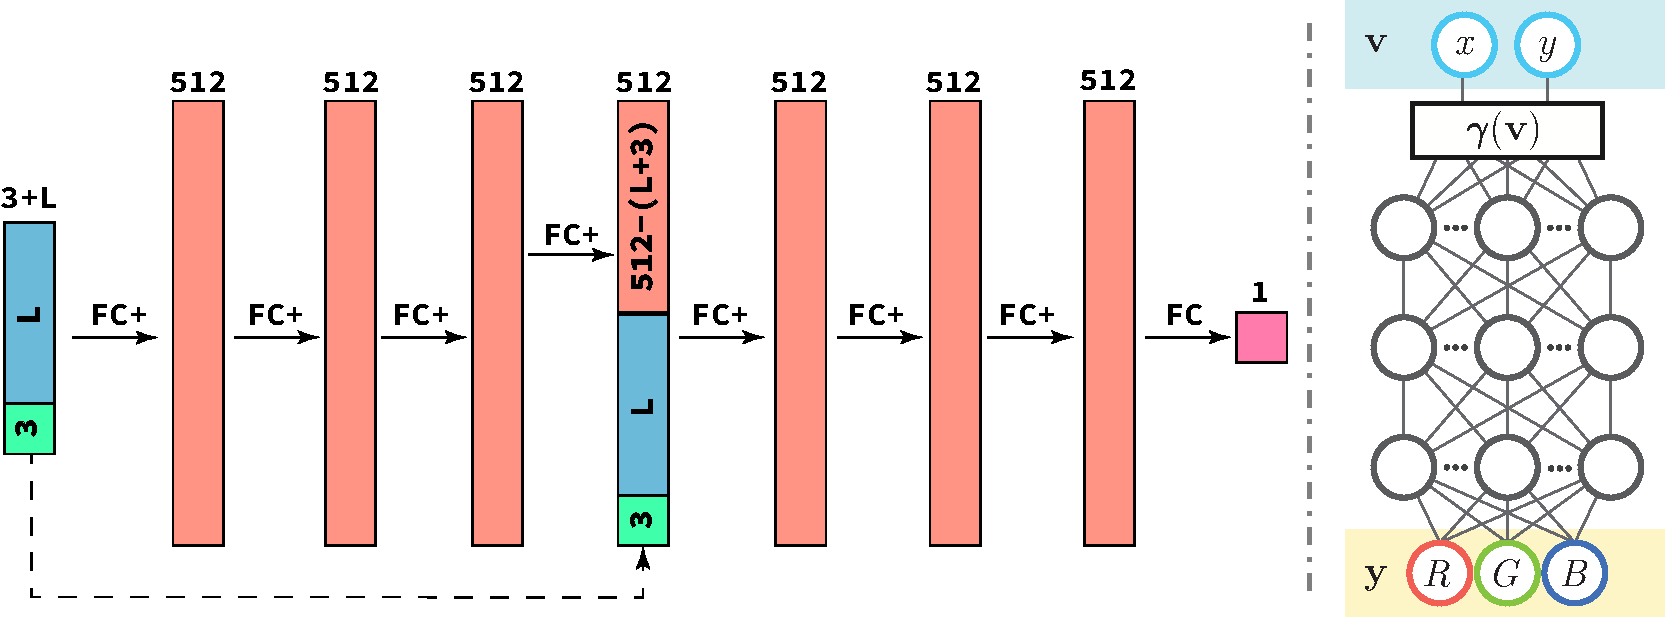
\includegraphics[width=0.8\textwidth]{imgs/arch.pdf}
    \caption{(左) MLP架构~\cite{gropp2020implicitgeometricregularizationlearning}, (右) MLP with Fourier features架构~\cite{tancik2020fourierfeaturesletnetworks}。 实际使用的MLP架构基于左图进行扩大, 为10层, 每层768个神经元, 在第5层进行跳跃连接。MLP with Fourier features在输入层前增加了对输入坐标的傅里叶特征变换($3\to 128$). }
    \label{fig:arch}
\end{figure}
如~\cref{fig:arch} 所示, 实际使用了10层的 MLP, 每层包含768个神经元, 在第5层进行了跳跃连接, 架构参考了 IGR~\cite{gropp2020implicitgeometricregularizationlearning} 使用 geometry initialization, 细节见 \texttt{model.py}.
MLP with Fourier features 的架构使用相同的 MLP, 但是在输入层前增加了对输入坐标的傅里叶特征变换, 将输出的3维坐标 $(x,y,z)$ 转换为128维的傅里叶特征, 参考了~\cite{tancik2020fourierfeaturesletnetworks} 实现, 代码见下:
\begin{minted}[bgcolor=LightGray]{python}
    class GaussianFourierFeatureTransform(nn.Module):
        def __init__(self, num_input_channels=3, mapping_size=64, scale=5):
            super().__init__()

            self._num_input_channels = num_input_channels
            self._mapping_size = mapping_size
            self._B = torch.randn((num_input_channels, mapping_size)) * scale
            self.output_dim = 2 * mapping_size

        def forward(self, x):
            """
            x: Point cloud coordinates of shape [B, 3]
            returns: Fourier features of shape [B, 2*mapping_size]
            """
            _, channels = x.shape
            x = x @ self._B.to(x.device)
            x = 2 * np.pi * x
            return torch.cat([torch.sin(x), torch.cos(x)], dim=1)
\end{minted}
MLP 和 MLP with Fourier features 的参数量/模型文件大小均为 21.3 MB, 实际参数量二者差别不大.

\subsection{训练策略与细节}
\paragraph{损失函数.} 参考作业文档, 记 $\tilde{F}(q) := \text{MLP}(q)$ 为 MLP 对于输入点 $q$ 的预测 SDF, $F(q)$ 为 ground truth SDF, $\nabla_q \tilde{F}(q)$ 和 $\nabla_q F(q)$ 分别为 MLP 和 ground truth 对于输入点 $q$ 的梯度. 损失函数定义为:
\begin{equation}
    \mathcal{L} = \lambda_{\text{sdf}} \cdot \mathcal{L}_{\text{sdf}} + \lambda_{\text{grad}} \cdot \mathcal{L}_{\text{grad}}
\end{equation}
其中
\begin{gather}
    \mathcal{L}_{\text{sdf}} = \frac{1}{N} \sum_{i=1}^{N} \left\| \tilde{F}(q_i) - F(q_i) \right\|^2_2, \quad\mathcal{L}_{\text{grad}} = \frac{1}{N} \sum_{i=1}^{N} \left\| \nabla_q \tilde{F}(q_i) - \nabla_q F(q_i) \right\|^2_2.
\end{gather}
注: 参考IGR~\cite{gropp2020implicitgeometricregularizationlearning} 还尝试了 eikonal norm loss, 在经过测试效果不好, 这里不赘述.

\paragraph{数据集.} 对于 MLP 由于输入的维度只有3维, MLP具有连续的特点, 我在实验中直接使用了点云数据进行训练, 测试效果可以恢复出较好的表面形状, 且在空间中未出现明显的 artifacts.
对于 MLP with Fourier features, 由于输入的维度为128维, 我使用了点云数据混合采样点, 单次采样的比例为$\text{点云}:\text{采样点} = 2:3$. 

\paragraph{详细配置.} 学习率、优化器、训练轮数、超参数的设置等详细设置见~\cref{tab:params}. 两个方法训练过程中均使用了Adam优化器, 学习率 scheduler 均使用 \texttt{CosineAnnealingLR(eta\_min=1e-6)}.
对于MLP with Fourier features, \texttt{fourier\_mapping\_size = 64}, \texttt{fourier\_scale = 5.0}.
\begin{table}[htbp]
    \centering
    \begin{tabular}{cccccccc}
        \toprule
        \textbf{Methods} & \textbf{学习率} & \textbf{优化器} & \textbf{单次采样数} & \textbf{训练轮数} & $\lambda_{\text{sdf}}$ & $\lambda_{\text{grad}}$ & \textbf{训练用时/mins} \\
        \midrule
        \textbf{MLP} & $10^{-4}$ & Adam & 20000 & 60000& 1.0 & 0.5 & 83 \\
        \textbf{MLP w/ Fourier} &  $2 \times 10^{-4}$ & Adam & 25000 & 100000& 2.0 & 0.5 & 197\\
        \bottomrule
    \end{tabular}
    \caption{训练超参数和用时对比, 实验在单卡 NVIDIA RTX 4090D 进行.}
    \label{tab:params}
\end{table}



\begin{figure}[htbp]
    \centering
    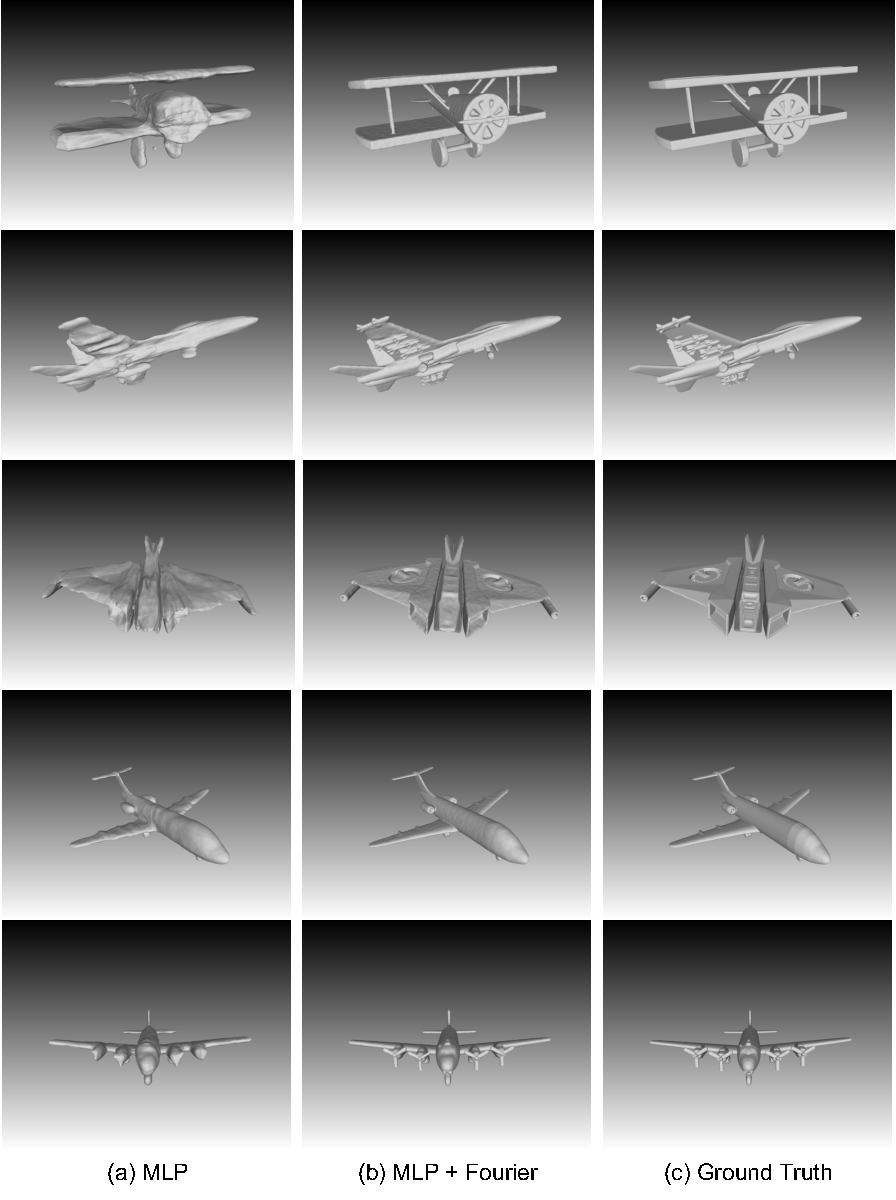
\includegraphics[width=\textwidth]{imgs/result.pdf}
    \caption{MLP 和 MLP with fourier features 的重建结果。放大查看细节。只有 MLP 生成的结果比较模糊且有较多细节缺失, 而使用 MLP with fourier features 生成的结果包含更多高频细节。}
    \label{fig:result}
\end{figure}

\subsection{测试细节}
\paragraph{后处理.} 由于MLP with Fourier features 的输入维度较高, 对于一两个物体经过训练后空间中会残留极少量的无意义碎块, 
在测试时, 通过 Marching Cubes 得到Mesh后, 只保留了最大的 connected component, 以去除这些碎块. 代码如下:
\begin{minted}[bgcolor=LightGray]{python}
    components = saved_mesh.split(only_watertight=False)
    if components:
        # Find the largest component by number of faces
        largest_component = max(components, key=lambda component: len(component.faces))
        saved_mesh = largest_component
    else:
        print("No components found or mesh is empty after split.")
\end{minted}
当然有其他后处理方式, 比如设定一个阈值, 只保留大于该阈值的 connected component. 实验中采取了上述方式, 效率比较高. 
注意\textbf{后处理只在 MLP with Fourier features 上进行}. MLP 由于高频细节较少, 部分物体会断开, 我选择直接使用 Marching Cubes 得到的 Mesh.

\paragraph{Marching Cubes.} 直接调用了\texttt{skimage.measure.marching\_cubes}, 而后用 trimesh 保存为 \texttt{.obj} 格式.
可以通过传入命令行 \texttt{--level} 参数来设置 Marching Cubes 的 level.

\paragraph{测试用时.} 当 \texttt{grid\_size} 设置为 256 时, 两个方法的测试用时在 5-6 秒. 当 \texttt{grid\_size} 设置为 512 时, 两个方法的测试用时在 40-50 秒, 后处理的耗时不大. 
最终保存下来的结果均使用了 \texttt{grid\_size = 512}, 以保证更高的精度.

\section{结果分析与讨论}
与 ground truth 相比, 只使用MLP的效果只能恢复出粗略的表面形状, 在 \cref{fig:result} 第一行的飞机模型中, 上下两层的连杆、螺旋桨等细节均未能恢复出来, 高频细节存在较多的缺失, 整体效果较差. 在训练过程中发现损失函数快速收敛且 $\mathcal{L}_{\text{sdf}}$ 下降到较小的值, 单纯通过增大训练步数不能够明显改善高频细节的恢复, 可能可以通过进一步增大模型或选择更精细的设计来改善结构的恢复. 限于时间原因没有进一步尝试.

使用 MLP with Fourier features 的方法能够恢复出更为精细的表面形状, 包含更多的高频细节, 较为接近 ground truth, 达到了预期的效果. 由于模型大小的限制, 以及没有设置更大的 Fourier features 的维度, 仍然存在一些更精细的高频细节的缺失, 例如第三行的飞机背部的纹理还存在模糊的情况, 以及最后一行飞机螺旋桨的棱角较为的平滑 等等. 但相较于 MLP 的方法, 整体效果有了明显的提升.

\bibliographystyle{plain} 
\bibliography{ref} 

\end{document}